\documentclass[12pt]{article}
\usepackage[margin=1in]{geometry} 
\usepackage{amsmath,amsthm,amssymb}
\usepackage{enumerate}
\usepackage{latexsym}
\usepackage{xparse}
\usepackage{minted}
\usepackage{hyperref}
\usepackage{graphicx} % Allows including images

\begin{document}

%%%%%%%%%%%%%%%%%%%%%%%%%%%
%%%%%%%% YO CANER %%%%%%%%%
%%%%%%%%%%%%%%%%%%%%%%%%%%%
%
% Here's the report requirements, as listed on canvas.iu.edu:
%
% You final project will include a written report, the source code for your
% compiler (on github), and the tests for your compiler.
%
% The written report should be 3-5 pages for undergraduates and 5-7 pages for
% graduate students. The report should include the following:
%
%   * What problem does your project solve? Or put another way, provide
%     documentation to a hypothetical user of your compiler regarding what your
%     project does for them, without discussing implementation details. Or put
%     yet another way, what are the goals of your project? This part of your
%     report could include example programs, syntax definitions, and definitional
%     interpreters.
%
%   * How does your project solve the problem? Give an overview of your
%     implementation and then discuss the most important details, which should
%     include both the trickiest parts but also the most important parts in
%     terms of having your implementation achieve its stated goals.
%
%   * Provide evidence that your project achieves its goals. This is called an
%     "evaluation". Describe any tests, experiments, or reasoning that you have
%     conducted to evaluate whether your implementation meets your stated goals.
%
%   * Clearly describe which goals have been achieved at the time of turning in
%     your project and which goals were unfinished.
%
%%%%%%%%%%%%%%%%%%%%%%%%%

\title{Tail-call optimization in $R_5$\vspace{-2ex}}
\author{Caner Derici and Ryan Scott} 
 
\maketitle

(\emph{Nota bene}: The code for this project is located at
\url{https://github.iu.edu/cderici/P523/tree/tail-call-optimization}. Our changes
were regression-tested against all of the original tests for $R_1$ through
$R_7$ in the \verb+tests/+ subdirectory, and we also added new tests, prefixed
with \verb+tco_+, to test our new additions.)

\begin{abstract}
  Tail-call elimination is an important optimization that
  functional languages heavily rely upon. It is based on the
  observation that a stack frame for a function call in a
  tail position can be eliminated by reusing the caller's frame. This
  makes tail recursion computationally equivalent to
  looping constructs (e.g. \verb+for+, \verb+while+) in imperative languages.

  We implemented tail-call elimination (TCO) on $R_5$ by making
  functions jump to the callee in the assembly level instead of making
  regular function calls, resulting in manual handling of the stack
  space. This allowed us to be able to reuse the same stack space for
  function calls, which essentially kept the space complexity at a
  constant factor. We also had to change the closure representation,
  which allows us to handle higher-order functions as well.
\end{abstract}

\section{Tail Calls}

A tail call is a function call in a tail position inside of a
function. A tail position is a fixed syntactic region of code that
signifies the idea of a ``last action of a function''. For example,
consider the following structurally recursive factorial function.

\begin{minted}[fontsize=\small]{Scheme}
  (define (fact n)
    (cond
      [(<= n 1) 1]
      [else (* n (fact (sub1 n)))]))
\end{minted}

The \verb+(fact (sub1 n))+ call inside of this function is \emph{not} in
a tail position. For example, when \verb+(fact 5)+ is invoked, the result of
the recursive call \verb+(fact (sub1 5))+ has to be multiplied with \verb+5+,
i.e. there's still something to do after the function
call. Because of this, we cannot overwrite the stack frame of \verb+(fact 5)+,
since we still have to keep the \verb+5+ until after \verb+(fact (sub1 5))+
returns (to multiply with it).

However, consider the following tail-recursive factorial function.

\begin{minted}[fontsize=\small]{Scheme}
  (define (fact-tail n acc)
    (cond
      [(<= n 1) acc]
      [else (fact-tail (sub1 n) (* n acc))]))
\end{minted}

Now the only action that a \verb+(fact 5 1)+ call will perform with the
result of \verb+(fact 4 5)+ is to return it. The key observation here is
that the results of \verb+(fact 5 1)+ and \verb+(fact 4 5)+ (and all the
subsequent calls in the computation sequence) are the same. Figure~1
shows the stack progression along with the return values for each function
invocation.

\begin{figure}[htb!]
  \centering
  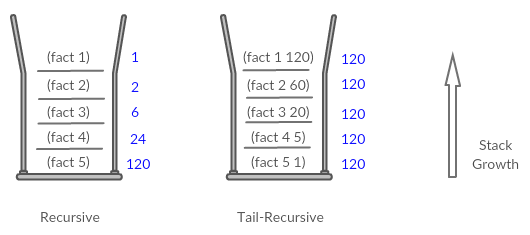
\includegraphics[scale=0.5]{stack.png}
  \caption{Stack Progressions of Regular and Tail Recursive Calls}
\end{figure}

This observation is the central idea behind tail-call elimination,
as the two subsequent tail calls can use the same stack frame. In a
recursive function, this essentially keeps overwriting the stack frame
of the first call, making the whole computation safe-for-space.

\section{Function calls in R5}
$R_5$, as originally defined in its reference implementation, doesn't take into
account whether function calls are in tail position, so it is completely oblivious to
any possibility of reusing the stack for tail calls. An unforunate consequence of this design
is that it is quite easy to define recursive $R_5$ functions that use up all available
stack space. Real-life examples of such functions include deeply tail-recursive functions
and infinite loops, e.g.,

\begin{minted}[fontsize=\small]{Scheme}
(define (explosion [n : Integer]) : Integer
  (explosion (+ n 1)))

(explosion 0)
\end{minted}

Without TCO, the generated assembly code for this function
will essentially be an infinite sequence of
\verb+callq+s and \verb+subq+s on the stack pointer, resulting in an
explosion of stack frames (hence the name). This is a problem. Not only does this
$R_5$ not meet the requirements of the Scheme report (which requires implementations
to be tail-recursive), but we can't even make infinite loops that are \emph{infinite}!

\section{Project goals}

When we first proposed this project, we divided up the work into three milestones,
in order of increasing difficulty:

\begin{enumerate}
 \item Apply tail call optimization only to first-order functions which use
       immediate tail recursion.
 \item Apply tail cail optimization to first-order functions that are mutually
       tail-recursive.
 \item  Apply tail cail optimization to all tail cails, even those involving
        higher-order function arguments and lambdas.
\end{enumerate}

We were confident in our ability to complete 1 and 2, but not as certain whether
we could successfully complete 3. In our original estimate, we believed that
implementing 3 correctly would involve applying inter-procedural static analysis
to determine which code paths one could go through in a program. However, we
realized that achieving 3 was much simpler if we adopted a strategy of storing
multiple labels in a closure (which we detail in the following section).

This approach turned out to work extremely well in $R_5$, and required none of the
fancy static analysis that we were afraid to implement. As a result, we successfully
completed all three milestones.

\section{Code changes}
Caner

\section{Measuring the benefits of TCO}

To instill a sense of appreciation for how much time and space TCO saves when running
compiled programs, we developed two microbenchmarks designed to demonstrate the benefits
of TCO. The first such microbenchmark is the Ackermann function $A$, which is defined
mathematically as follows:

$$
A(m, n) = \begin{cases}
  n+1               & \mbox{if } m = 0 \\
  A(m-1, 1)         & \mbox{if } m > 0 \mbox{ and } n = 0 \\
  A(m-1, A(m, n-1)) & \mbox{if } m > 0 \mbox{ and } n > 0.
\end{cases}
$$

$A$ is of particular interest to computer scientists not only
because of its interesting computability properties, but also because it can lead
to extremely deep levels of recursion, making it useful as a performance benchmark.
Note that while we can define $A$ straightforwardly in $R_5$, it doesn't show off
the benefits of TCO as much as it could due to the call to $A$ in non-tail position
in the third case. Therefore, the program we will benchmark will be converted
to continuation-passing style to leverage more tail calls:

\begin{minted}[fontsize=\small]{Scheme}
(define (ackermann-cps [cont : (Integer -> Integer)]
                       [m : Integer] [n : Integer]) : Integer
  (if (eq? m 0) (cont (+ n 1))
      (if (eq? n 0)
          (ackermann-cps cont (+ m (- 1)) 1)
          (ackermann-cps
            (lambda: ([x : Integer]) : Integer (ackermann-cps cont (+ m (- 1)) x))
            m (+ n (- 1))))))
(define (ackermann [m : Integer] [n : Integer]) : Integer
  (ackermann-cps (lambda: ([x : Integer]) : Integer x) m n))
(ackermann 3 5)
\end{minted}

We compiled this program with two versions of our $R_5$ compiler---
one with TCO enabled, and one without it---and ran the compiled code
using the \verb+/usr/bin/time+ program on Linux.

The results for the compiler with TCO:

\begin{minted}[fontsize=\small]{text}
$ /usr/bin/time -v ./a.out 
253     ...
        Elapsed (wall clock) time (h:mm:ss or m:ss): 0:00.00
        ...
        Maximum resident set size (kbytes): 3252
        ...
        Minor (reclaiming a frame) page faults: 525
        ...
\end{minted}

The results for the compiler without TCO:

\begin{minted}[fontsize=\small]{text}
$ /usr/bin/time -v ./a.out 
253     ...
        Elapsed (wall clock) time (h:mm:ss or m:ss): 0:00.00
        ...
        Maximum resident set size (kbytes): 8560
        ...
        Minor (reclaiming a frame) page faults: 1848
        ...
\end{minted}

The difference is clear: enabling TCO saves about 5.3 MB worth of RAM usage, and
prevents 1323 page faults! From a memory perspective, TCO is an obvious win.

What is suprising, however, is that both programs run nearly instantly. We would
have expected the code with TCO to run a little slower, but in practice, this
does not turn out to be the case. In face, even with the following microbenchmark
designed to churn through millions of function calls:

\begin{minted}[fontsize=\small]{Scheme}
(define (make-your-cpu-get-hot [x : Integer] [y : Integer]) : Integer
  (if (eq? 0 x)
      42
      (make-your-cpu-get-hot (+ x (- y)) y)))
(let ([a-little-warmer (lambda: () : Integer (make-your-cpu-get-hot 100000 1))])
  (let ([a0   (a-little-warmer)])
  ...
  (let ([a499 (a-little-warmer)])
    (a-little-warmer))...))
\end{minted}

Both compilers, with and without TCO, produce code which finishes in less than one
second. We learned that adjusting the stack pointer is not as computationally
expensive as we had originally thought. Still, from the perspective that fewer
x86 instructions = faster runtime, TCO is certainly preferable, and from a
memory usage perspective, there is demonstrable evidence that TCO wins.

\section{Design considerations and future work}

We wish to emphasize that while our work successfully adds TCO to $R_5$, it is by
no means an \textit{optimal} solution. In particular, we made an extreme simplification
by requiring that all top-level \verb+define+s allocate (and deallocate) the exact
same amount of stack space. Although this makes it possible for a series of tail calls
to successfully finish in any \verb+define+d function, it is also quite wasteful, since
all functions now must allocate as much stack space as possible.

It is difficult to envision a robust solution to this problem, since given the existence
of higher-order functions, it can be difficult to know statically all possible paths
through \verb+define+d functions. One idea is to change the generated code such that
closures also store how much stack space the underlying function requires, and creating
a different conclusion for tail calls that \verb+addq+s \verb+%rsp+ an amount equal
to the stack space number inside the closure. There would have to be an additional
runtime cost associated with checking if a function should \verb+jmp+ to the normal
conclusion or the special tail-call conclusion, but the cost may be worthwhile
given the amount of memory this technique could save.

Another area for improvement is in the generated code for closures themselves.
Currently, closures have two separate entries for non-tail-call labels (e.g.,
\verb+foo+) and tail-call label (e.g., \verb+fooEntry+). This seems like a code
smell, since we always know that a tail-call label is just the original label with
the suffix \verb+Entry+. It may be possible, using some assembly trickery, to
retrieve the non-tail-call label and concatenate \verb+Entry+ on the end to
synthesize the tail-call label. If such a thing is possible, it would allow us
to save 8 bytes per closure.

Space considerations notwithstanding, our project proves that TCO is inside the
realm of possibility for $R_5$, and it can successfully coexist with more advanced
language features like higher-order function arguments and lambdas. This is good
news, because it means that even first-time compiler authors can successfully
create a Scheme that adheres to the specification!

\end{document}
